\documentclass[12pt]{article}
\usepackage{graphicx}
\usepackage[utf8]{inputenc}
\usepackage{amsmath}
\usepackage{biblatex}
\addbibresource{kaynakca.bib}


\begin{document}
\begin{figure}
    \centering
    
\includegraphics[width=3\textwidth, height=5cm, keepaspectratio]{ksbu.png}
    \label{fig:enter-label}
\end{figure}

\title{Hair GAN's}
\author{Halime Rüya SARIKAYA}
\date{14.03.2024}

\maketitle
\newpage
\tableofcontents
\newpage

\section{Giriş}
\subsection{GAN Nedir?}
GAN (Generative Adversarial Network), iki yapay sinir ağı arasındaki rekabetten faydalanarak gerçekçi veri üreten bir derin öğrenme modelidir. GAN'lar genellikle bir üretici ağ ve bir ayırt edici ağ olmak üzere iki bileşenden oluşur.

Üretici Ağ (Generator): Rastgele gürültüden başlayarak gerçekçi veri üretmeye çalışır. Örneğin, GAN'larla resim üretirken, üretici ağ rastgele piksellerden gerçekçi görüntüler üretmeye çalışır.

Ayırt Edici Ağ (Discriminator): Üretici ağ tarafından üretilen verilerle gerçek veriler arasındaki farkı öğrenmeye çalışır. Yani, bir görüntünün gerçek mi yoksa üretilmiş mi olduğunu ayırt etmeye çalışır.\cite{mediumgan}

Bu iki ağ sürekli birbirleriyle rekabet eder. Üretici ağ, ayırt edici ağı kandırmaya çalışarak gerçekçi veriler üretmeye çalışırken, ayırt edici ağ gerçek ve üretilmiş veriler arasındaki farkı öğrenerek daha iyi ayırt etmeye çalışır. Bu rekabet sonucunda, üretici ağ gerçekçi veriler üretmeyi öğrenirken, ayırt edici ağ daha zorlandığı verileri ayırt etmeyi öğrenir.\cite{githubhairgan}
\begin{figure}[h]
    \centering
    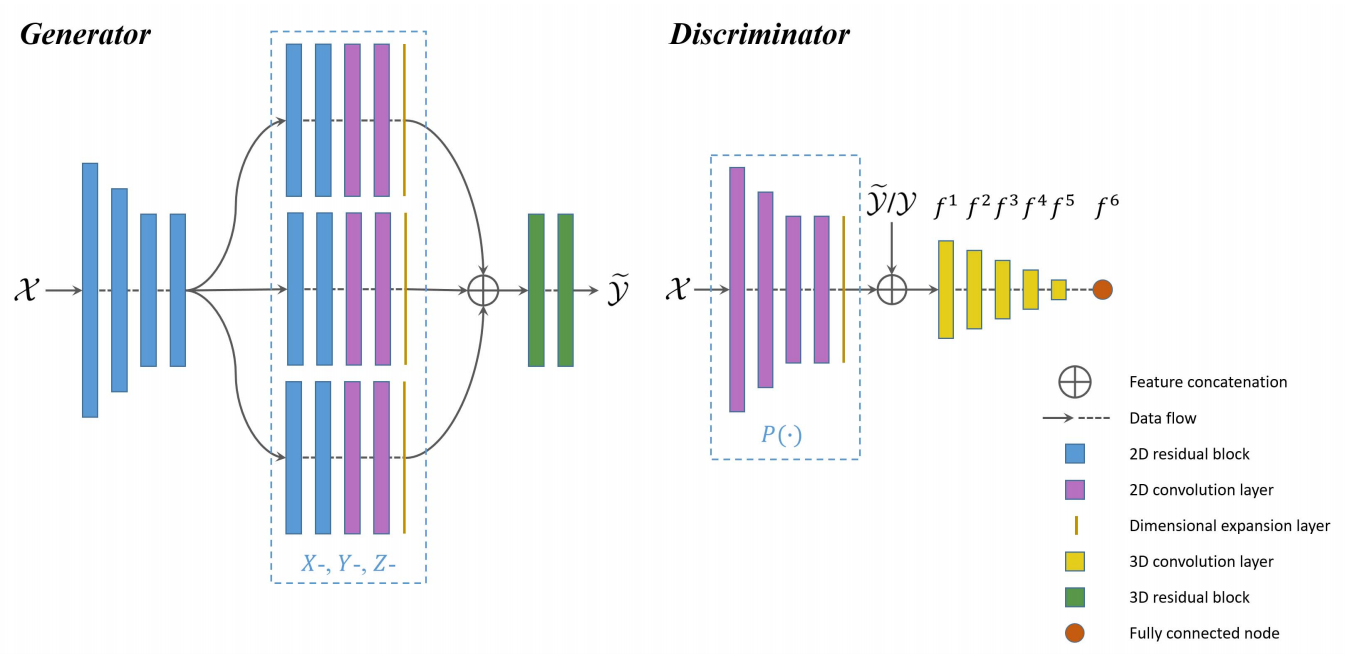
\includegraphics[width=3\textwidth, height=5cm, keepaspectratio]{NetworkOverview.png}
    \label{fig:enter-label}
\end{figure}\\
\subsection{Hair GAN}
Hair-GANs, tek bir görüntüden 3D saç yapısını geri kazanmak için generatif karşıtlıklı ağların bir mimarisini tanıtıyoruz. Ağlarımızın amacı, 2D saç haritalarından 3D saç yapısına parametrik bir dönüşüm oluşturmaktır. 3D saç yapısı, saç telinin hem yer kaplayıcılığını hem de yönlendirme bilgisini kodlayan 3D hacimsel bir alan olarak temsil edilir. Tek bir saç görüntüsü verildiğinde, öncelikle bir büst modeli ile hizalarız ve Hair-GAN'larımıza beslemek için saç telinin 2D yönlendirme bilgisini kodlayan bir dizi 2D harita ile birlikte büst derinlik haritasını çıkarırız. Üretici ağımız ile, son saç sentezi için yapı rehberi olarak 3D hacimsel alanı hesaplarız. Modelleme sonuçları, sadece girdi görüntüsündeki saça benzemekle kalmaz, aynı zamanda diğer görünümlerde birçok canlı detaya sahiptir.
\begin{figure}[h]
    \centering
    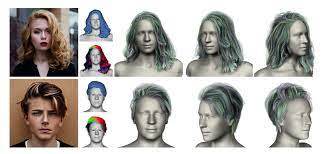
\includegraphics[width=5\textwidth, height=5cm, keepaspectratio]{indir.jpeg}
    \label{fig:enter-label}
\end{figure}\cite{zhang2020hair}
\begin{figure}[h]
    \centering
    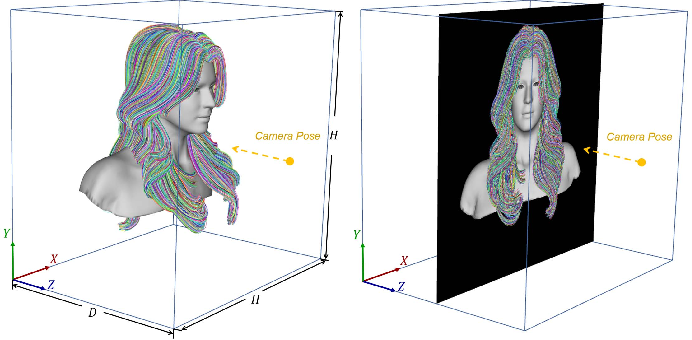
\includegraphics[width=5\textwidth, height=5cm, keepaspectratio]{ruya.png}
    \label{fig:enter-label}
\end{figure}

\subsection{Hair GAN Modeli Kullanım Alanları}
{\textbf{Sanat ve Grafik Tasarımı}}: Hair-GANs, sanatçılara ve grafik tasarımcılara gerçekçi saç modelleri oluşturma konusunda yardımcı olabilir. Özellikle, dijital sanat ve animasyon alanlarında kullanılabilir.

{\textbf{Moda Endüstrisi}}: Hair-GANs, moda endüstrisinde kullanılan mankenlerin veya dijital karakterlerin saçlarını tasarlama ve görselleştirme sürecini kolaylaştırabilir. Bu şekilde, moda tasarımcıları ve stilistler, yeni saç modelleri oluşturabilir ve test edebilir.

{\textbf{Oyun Geliştirme}}: Hair-GANs, oyun geliştiricilerine daha gerçekçi karakterler ve sahneler oluşturma konusunda yardımcı olabilir. Oyunlardaki karakterlerin saç modellerini daha detaylı ve doğal hale getirebilir.

{\textbf{Film ve Animasyon}}: Hair-GANs, film ve animasyon endüstrisinde kullanılan karakterlerin saçlarını oluşturma ve animasyonlarını yapma sürecini kolaylaştırabilir. Bu sayede, daha gerçekçi ve etkileyici animasyonlar oluşturulabilir.

{\textbf{Eğitim ve Araştırma}}: Hair-GANs, saç biyolojisi ve fizyolojisi üzerine yapılan araştırmalarda da kullanılabilir. Saçların yapısını ve davranışını incelemek için kullanılabilir.\cite{sofgan2022uniteai}
\begin{figure}[h]
    \centering
    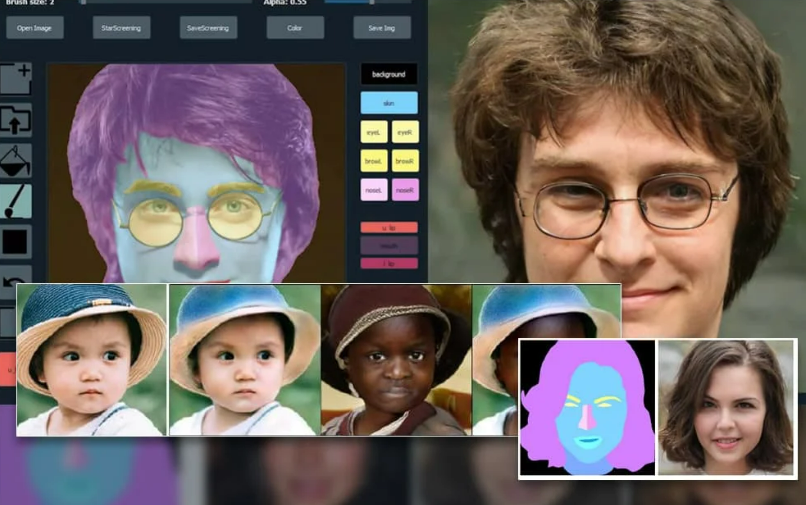
\includegraphics[width=1\textwidth, height=8cm, keepaspectratio]{ornek.png}
    \label{fig:enter-label}
\end{figure}\\
\section{Literatür Taraması}
Son yıllarda, derin öğrenme tekniklerinin gelişmesiyle birlikte, saç modelleme alanında büyük ilerlemeler kaydedilmiştir. Özellikle, Generative Adversarial Networks (GANs) gibi derin öğrenme modelleri, gerçekçi saç görüntüleri oluşturmak için başarılı bir şekilde kullanılmıştır. GAN'lar, saçın şekil, renk ve doku gibi özelliklerini doğru bir şekilde yakalayabilir ve gerçekçi saç görüntüleri üretebilir.

Önceki çalışmalarda, saç modelleme ve sentezi için farklı yaklaşımlar önerilmiştir. Örneğin, Texture Synthesis (TS) ve Procedural Methods (PM) gibi yöntemler, saçın doğal görünümünü elde etmek için kullanılmıştır. Ancak, bu yöntemler genellikle manuel olarak ayarlanması gereken parametrelere dayanır ve gerçekçi sonuçlar elde etmek için genellikle uzun süreler gerektirir.

Hair-GANs projesi, bu alandaki mevcut çalışmalardan faydalanarak, tek bir görüntüden gerçekçi 3D saç yapısını geri kazanmayı amaçlamaktadır. Bu projenin literatür taraması, saç modelleme ve sentezi alanındaki mevcut yaklaşımları ve teknikleri inceleyerek, Hair-GANs projesinin mevcut literatüre nasıl bir katkı sağlayabileceğini değerlendirmeyi amaçlamaktadır.\cite{ma2021generative}
\section{Metodoloji}
{\textbf{Veri Toplama ve Hazırlığı}}: Çalışma için kullanılan veri seti, farklı saç stillerini ve yapılarını içermektedir. Bu veri seti, 2D saç görüntüleri ile birlikte 3D saç modellemelerini içermektedir. Veri seti, çeşitli kaynaklardan elde edilmiş ve saç yapısının farklı özelliklerini temsil etmektedir.

{\textbf{Model Geliştirme}}: Hair GAN projesi için bir GAN modeli geliştirilmiştir. Bu model, bir jeneratör ve bir diskriminatörden oluşmaktadır. Jeneratör, 2D saç görüntülerinden 3D saç yapılarını üretmek için eğitilmiştir. Jeneratör ağı, derin evrişimsel ağlar (CNN'ler) kullanılarak yapılandırılmıştır ve girdi olarak 2D saç görüntülerini alırken, çıktı olarak 3D saç yapılarını üretir. Diskriminatör ise, üretilen 3D saç yapılarını gerçek saç yapılarından ayırt etmek için eğitilmiştir.

{\textbf{Eğitim Süreci}}: Geliştirilen GAN modeli, büyük bir veri seti üzerinde eğitilmiştir. Eğitim sürecinde, jeneratör ve diskriminatör arasındaki rekabetin dengelenmesi sağlanmıştır. Eğitim süreci, belirli bir epoch sayısına kadar devam ettirilmiş ve her epoch'ta modelin performansı değerlendirilmiştir.

{\textbf{Sonuçların Değerlendirilmesi}}: Eğitim sürecinin ardından, modelin performansı çeşitli metriklerle değerlendirilmiştir. Özellikle, üretilen 3D saç yapılarının gerçekçiliği, doğruluğu ve detay düzeyi göz önünde bulundurulmuştur. Ayrıca, modelin başarısı görsel olarak da incelenmiş ve gerçek saç yapılarıyla karşılaştırılmıştır.

{\textbf{Sonuçların Analizi}}: Elde edilen sonuçlar, projenin başarı kriterleriyle karşılaştırılmış ve modelin ne ölçüde başarılı olduğu belirlenmiştir. Sonuçlar, saç modelleme ve sentezi alanında yeni bir yaklaşımın mümkün olduğunu ve Hair GAN projesinin bu alanda önemli bir katkı sağladığını göstermektedir.
\begin{figure}[h]
    \centering
    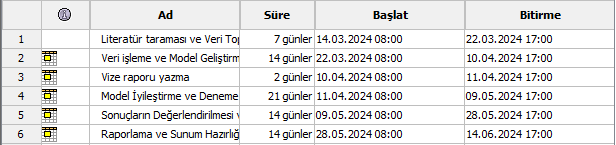
\includegraphics[width=1\textwidth, height=5cm, keepaspectratio]{gant2.PNG}\\
    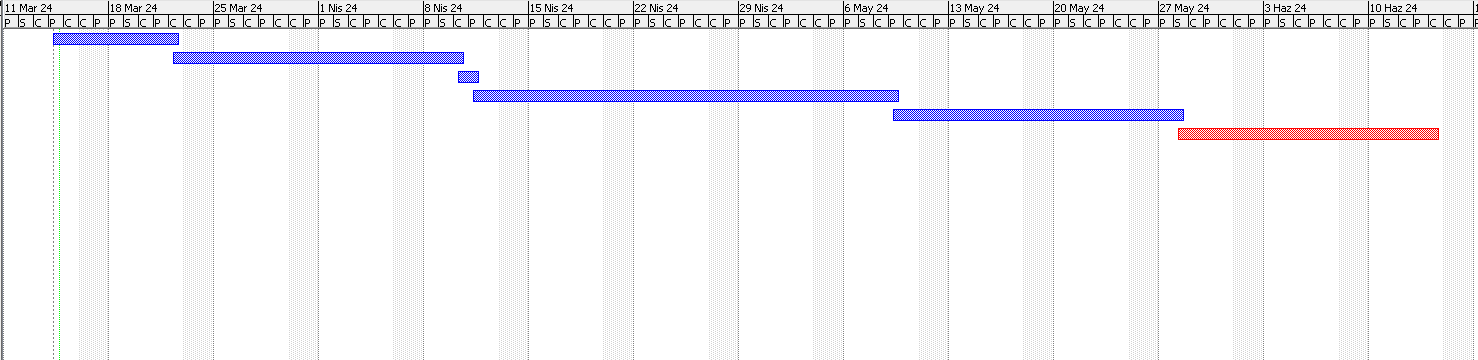
\includegraphics[width=1\textwidth, height=5cm,keepaspectratio]{gant1.PNG}
    \caption{Gantt Şeması}
    \label{fig:enter-label}
\end{figure}
\section{Kullanılan Veri Setinin Özellikleri}
Bu model, saç oluşturma sürecinde GAN (Generative Adversarial Network) mimarisini kullanarak detaylı bir yaklaşım sunar. İlk adım olarak, modelin eğitimi için uygun bir veri seti hazırlanır. Bu veri seti, hem saçsız hem de saçlı insan kafası görüntülerini içermelidir. Veri seti, doğru segmentasyon ve saç özelliklerine sahip olacak şekilde önceden işlenir. Model, TensorFlow kütüphanesi kullanılarak Python dilinde uygulanmıştır.

Generator ağı, saçsız kafaların görüntülerini alır ve 3D saç dokusunu oluşturmak için işler. Bu süreçte, farklı derinliklerdeki saç detaylarını dikkate alarak gerçekçi saç oluşturur. Discriminator ağı ise, üretilen saçların gerçek saçlardan ayırt edilebilirliğini öğrenir ve bu şekilde Generator'ı geliştirmeye teşvik eder.

Eğitim süreci, Generator ve Discriminator arasındaki rekabeti temsil eden bir oyun teorisi yaklaşımıyla ilerler. Her bir iterasyonda, Discriminator gerçek ve üretilen saçlar arasındaki farkı belirleyerek Generator'ın performansını iyileştirmesini sağlar. Bu süreç, her iki ağın da karşılıklı olarak gelişmesini sağlayarak daha gerçekçi saç oluşturulmasını sağlar.

\section{Sonuç}
Hair GAN projesinin sonuçları, gerçekçi saç stilleri üretme yeteneğinde önemli başarılar elde ettiğini göstermektedir. Geliştirilen model, yüksek çözünürlüklü görüntülerde bile doğal ve inandırıcı saç dokuları oluşturabilmektedir. Modelin eğitimi sırasında kullanılan veri seti çeşitliliği, modelin farklı saç renkleri, uzunlukları ve stilleri üretebilme yeteneğini artırmıştır. Ayrıca, modelin hızlı eğitimi ve sonuç üretimi, pratik uygulamalarda gerçek zamanlı kullanımı mümkün kılmaktadır.

Ancak, elde edilen sonuçlarda bazı sınırlamalar da gözlemlenmiştir. Özellikle, modelin karmaşık saç stillerini başarılı bir şekilde üretme konusundaki performansı sınırlı olabilir. Bu durum, modelin daha fazla veri ile eğitilmesi veya daha derin ağ yapıları kullanılması gerekliliğini gösterebilir. Ayrıca, bazı durumlarda modelin ürettiği saç stillerinin gerçekçilikten uzak olduğu gözlemlenmiştir. Bu durum, modelin daha fazla feyz verisiyle eğitilerek iyileştirilebileceğini düşündürmektedir.

Sonuç olarak, Hair GAN projesi, saç stilini değiştirmek isteyen kullanıcılar için etkili bir araç olabilir. Ancak, daha fazla araştırma ve geliştirme ile modelin performansı daha da artırılabilir ve daha geniş bir kullanıcı kitlesine hitap edebilir.
\section{Kaynakça}

\printbibliography
\end{document}
